\begin{enumerate}[label=\thesubsection.\arabic*,ref=\thesubsection.\theenumi]
%
 \item A fair six-faced dice, with the faces labelled ‘1’, ‘2’, ‘3’, ‘4’, ‘5’, and ‘6’, is rolled
    thrice. What is the probability of rolling ‘6’ exactly once?\hfill(AG 2025)
	\begin{multicols}{4}
 \begin{enumerate}
    \item $\frac{75}{216}$
    \item $\frac{1}{6}$
    \item $\frac{1}{18}$
    \item $\frac{25}{216}$
\end{enumerate}
\end{multicols}
\solution
From \eqref{eq:EE26BTECH11213-dice_uniform_pmf},
        \begin{align}
            P_{X_1}(k)=
                \begin{cases}
                    \frac{1}{6} &  k=1 \\
                    \frac{5}{6} & k=0\\
                \end{cases}
        \end{align}
       where $X_i$ represents the $i$th roll. 
Substituting $n=3,
p=\frac{1}{6}, 
q=\frac{5}{6}$,
in \eqref{eq:EE26BTECH11213-pmf-bern},
the desired probability is obtained as
    \begin{align}
	    \comb{3}{1}\frac{1}{6}\brak{\frac{5}{6}}^2
        =\frac{75}{216}.
    \end{align}
The following code simulates the result 
\begin{lstlisting}
codes/Probability.c
\end{lstlisting}
%
	\item If $a, b$, and $c$ are the roots of 
    \begin{align}
		2x^3 - 3x^2 + px - 1=0
       \label{eq:absum-root}
	\end{align}
		and sum of the two roots is 1, the value of $p$ is \hfill(AG 2025)
	\begin{multicols}{4}
\begin{enumerate}
    \item 2
    \item 1
    \item 3
    \item $\frac{1}{3}$
\end{enumerate}
\end{multicols}
%
    \solution
    Using the sum and product of roots from high school algebra and the given information, 
    \begin{align}
       \label{eq:absum}
	    a+b&=1
       \\
\label{eq:sum}
 a+b+c &=\frac{3}{2}
 \\
\label{eq:prod}
        abc&=\frac{1}{2}\\
\label{eq:pair}
        ab+bc+ac&=\frac{p}{2}
    \end{align}
From 
       \eqref{eq:absum}
       and
\eqref{eq:sum},
    \begin{align}
                               c=\frac{1}{2}, 
			       \label{eq:valofc}
		       \end{align}
\eqref{eq:pair}
can be expressed as
    \begin{align}
\frac{p}{2}	&=    \frac{abc}{c}+c\brak{a+b}=
\frac{1}{2c} + c
\\
        \implies p&=3
\label{eq:par-p}
    \end{align}
    upon 
    substituting
    from 
       \eqref{eq:absum},
\eqref{eq:prod}
       and
			       \eqref{eq:valofc}.
Using the Newton-Raphson method     
the difference equation for computing the root of 
       \eqref{eq:absum-root} is
\begin{align}
    x_{n+1}=x_n+\frac{2x^3-3x^2+3x-1}{6x^2-6x+3}   
    \end{align}
   from \eqref{eq:EE26BTECH11213-newton_raphson}.
    With an initial guess of 4, running this difference equation 6 times gives us the real root, which is $\frac{1}{2}$.
The following code verifies the result
in 
    \figref{fig:Newtonraphsonfig}.
\begin{lstlisting}
codes/raph.py
\end{lstlisting}
    \begin{figure}[htbp]
    \centering
    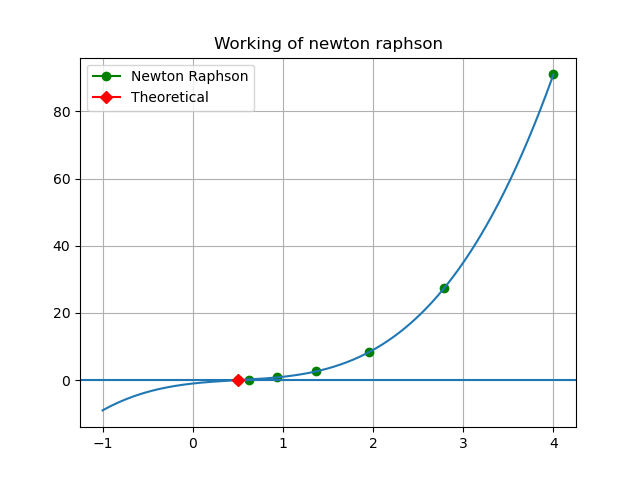
\includegraphics[width=0.7\textwidth]{figs/rson.png}
    \caption{The depiction of newton raphson method guessing the root}
    \label{fig:Newtonraphsonfig}
\end{figure}
\item If the matrix $\myvec{ x & -3 \\ 2 & x-5 }$ is singular, sum of the values of $x$ is     \hfill(AG 2025)   
	\begin{multicols}{4}
    \begin{enumerate}
    \item 5
    \item 6
    \item  0
    \item $-1$
\end{enumerate}
	\end{multicols}
%
\solution
Through row reduction, 
\begin{align*}
    \myvec{
        x& -3 \\
        2& x-5
    }
    \xleftrightarrow{R_2 \leftrightarrow R_1}
    \myvec{
        2& x-5 \\
        x& -3 
    }
    \xleftrightarrow{R_2 \leftarrow 2R_2 - xR_1}
	\myvec{
        2& x-5 \\
        0& -6-x^2+5x
        }    
\end{align*}
For the matrix to be singular, from Definition
			\ref{eq:EE26BTECH11202-singular-def},
\begin{align}
    x^2-5x+6=0
\end{align}
Hence, the sum of roots is 5.
The following code verifies the result
\begin{lstlisting}
codes/echelon.py
\end{lstlisting}
%
\item $\frac{s}{s^2+a^2}$ is the Laplace transform of \hfill(AG 2025)
    \begin{enumerate}
	\begin{multicols}{4}
    \item cos$\brak{at}$
    \item sin$\brak{at}$
    \item sinh$\brak{at}$
    \item cosh$\brak{at}$
%                
    \end{multicols}
    \end{enumerate}
%%    
\solution
From \eqref{eq:EE26BTECH11202-Laplace_5}, 
\begin{align}
\cos\brak{at}\system{L}\frac{a}{s^2+a^2}
\end{align}
%
\item The median of the following set of numbers: 154, 130, 144, 137, 156, 146, 138,
149, 160, 138 is:\hfill(AG 2025)
    \begin{enumerate}   
	\begin{multicols}{4}
    \item $145.0$
    \item $145.2$
    \item $151.0$
    \item $146.0$
    \end{multicols}
    %\item[SOL] NEED TO WRITE SOL!!!
    \end{enumerate}   
%
\solution
From the  
following codes, the median is obtained as 
145.0
\begin{lstlisting}
codes/Sorter.py
codes/Quicksort.c
\end{lstlisting}
\item The series 
    \begin{align}
\sum_{n=0}^{r} q^n =1+q+q^2+ \dots
\end{align}
 has the sum \hfill(AG 2025)
	\begin{multicols}{4}
    \begin{enumerate}
    \item $\frac{1}{1-q}$-$\frac{q^{r+1}}{1-q}$
    \item $\frac{1}{q-1}$+$\frac{q^{r+1}}{q-1}$
    \item $\frac{1}{1-q}$+$\frac{q^{r+1}}{1-q}$
    \item $\frac{1}{q-1}$
    %\item[SOL] NEED TO WRITE SOL!!! 
    \end{enumerate}
\end{multicols}
\solution
	From \eqref{eq:sumofgp},
    the desired sum is
    \begin{align}
        \frac{1-q^{r+1}}{1-q}=
        \frac{1}{1-q}-\frac{q^{r+1}}{1-q}        
    \end{align}
The following code verifies the result.
\begin{lstlisting}
codes/gp.py
\end{lstlisting}
\item The value of $\lim_{x\to 0}\frac{x\cos\brak{x}-\sin\brak{x}}{x^2\sin\brak{x}}$\hfill(AG 2025)
	\begin{multicols}{4}
    \begin{enumerate}
        \item $-\frac{1}{3}$
        \item $\frac{1}{3}$
        \item $3$
        \item$-3$
\end{enumerate}
\end{multicols}
        \solution
%        We use the idea of taylor series expansion (converges if $x<1$) to solve the problem.\\
        From  \eqref{eq:expansions},
       \begin{align}
        \frac{x\brak{\cos\brak{x}}-\sin\brak{x}}{x^2\sin\brak{x}}
        &=\frac{x(1-\frac{x^2}{2!} .....)-(x-\frac{x^3}{3!}.....)}{x^2(x-\frac{x^3}{3!}.....)}
	\\
    		&\approx \frac{(x-\frac{x^3}{2})-(x-\frac{x^3}{6})}{x^3(1-\frac{x^2}{6})}\\
        &=-\frac{\frac{1}{3}}{1-\frac{x^2}{6}}
	\\
	\implies \lim_{x\to 0}\frac{x\cos\brak{x}-\sin\brak{x}}{x^2\sin\brak{x}}
	&=-\frac{1}{3}.
       \end{align}
The following code generates
    \figref{fig:limit}.
\begin{lstlisting}
codes/Plottinglimit.py
\end{lstlisting}
\begin{figure}[htbp]
    \centering
    \includegraphics[width=0.7\textwidth]{figs/limitplot.png}
    \caption{}
    \label{fig:limit}
\end{figure}
\item If $u=x^4+y^4+3x^2y^2$, the value of $\left(x\frac{\partial{u}}{\partial{x}}+y\frac{\partial{u}}{\partial{y}}\right)^{-1}$\hfill(AG 2025)
	\begin{multicols}{4}
\begin{enumerate}
    \item $4u$
    \item $0$
    \item $\frac{1}{4u}$
    \item $2u$
    %\item[SOL] NEED TO WRITE SOL!!! 
\end{enumerate}
\end{multicols}
\solution
Since
\begin{align}
u\brak{\alpha x,\alpha y}=\alpha^4u\brak{\alpha x,\alpha y},
\\
    x\frac{\partial u}{\partial x}+y\frac{\partial u}{\partial y}=4u 
    \\
    \text{or, }
    \brak{x\frac{\partial u}{\partial x}+y\frac{\partial u}{\partial y}}^{-1}=\frac{1}{4u} 
\end{align}
from \eqref{eq:eulerhomo}.
\item  Given $y\brak{x=0}=0$ for the differential equation $\frac{dy}{dx}=3y+2e^x$, the value of $y$ at $x=0.3$ is \underline{\hspace{1cm}}. \hfill(AG 2025)
%
	\\
\solution
	From 
\eqref{eq:EE26BTECH11202-Laplace_1}
and
	\eqref{eq:EE26BTECH11202-Laplace-exp},
 \begin{align}
     sY\brak{s}&=3Y\brak{s}+2\frac{1}{s+1}
     \\
\implies     Y\brak{s}&=\frac{2}{\brak{s-1}\brak{s-3}}
    \\
    &=\frac{1}{s-3}-\frac{1}{s-1}
    \\
    \text{or, }
	y(x)&=\brak{e^{3x}-e^{x} }u(x)
\end{align}
by considering the inverse.
\begin{align}
	\therefore
    y\brak{0.3}=1.110
\end{align}
	From \eqref{eq:EE26BTECH11202-ED_1},
\begin{align}
y_{n+1}=y_{n}+h(3y_n+2e^n).
    \label{eq:Forwardeuler}
\end{align}
The following code computes 
    \eqref{eq:Forwardeuler}
    and generates
    \figref{fig:Forwardeuler}.
simulates the result:
\begin{lstlisting}
codes/diffeq.py
\end{lstlisting}
\begin{figure}[htbp]
    \centering
    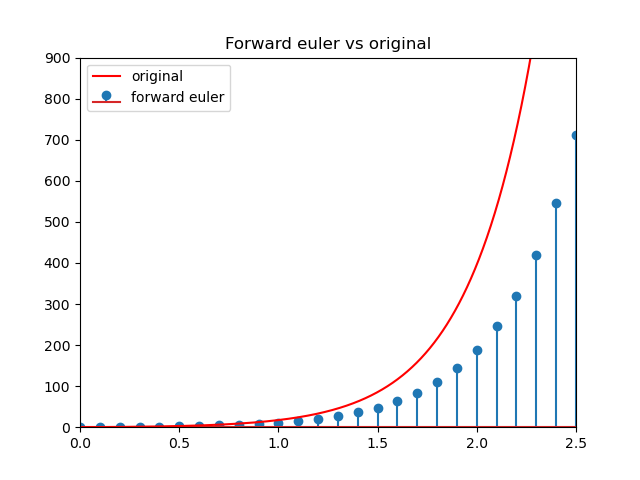
\includegraphics[width=0.5\textwidth]{figs/Euler.png}
    \caption{The plot depicting the divergence of forward euler from theory at large values}
    \label{fig:Forwardeuler}
\end{figure}
\end{enumerate}
%\end{document}
